\documentclass[12pt]{report}
\usepackage{GraphDefinitions}

\begin{document}

\def\grayopacity{0.055}
\def\ballsize{3pt} % Change the size of the balls
\def\seencolor{orange}
\def\seenx{543}
\def\seeny{340}
\def\seenz{500}
\def\calix{574}
\def\caliy{271}
\def\caliz{435}
\def\calicolor{blue}
\def\maxy{750}
\def\maxx{825}
\def\shadowopacity{0.4}
            
\begin{figure}[H]
    \centering
    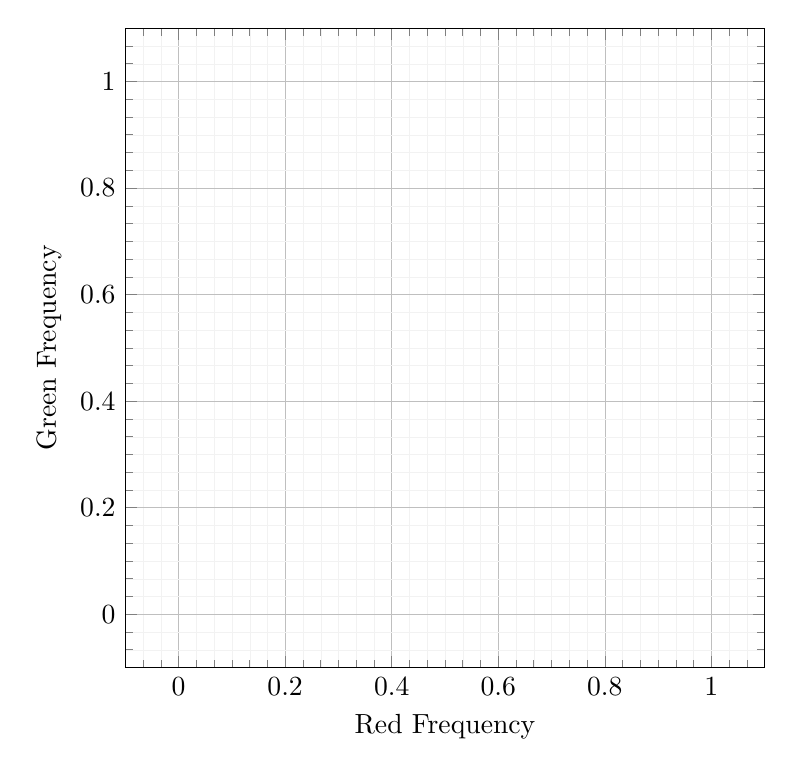
\begin{tikzpicture}
        \begin{axis}[
            xlabel={Red Frequency},
            ylabel={Green Frequency},
            zlabel={Blue Frequency},
            xlabel style={sloped like x axis}, % Make x label follow the x axis
            ylabel style={sloped like y axis}, % Make y label follow the y axis
            zlabel style={sloped}, % Make z label follow the z axis or make it vertical
            legend pos=north west,
            grid=both,
            grid style={line width=.1pt, draw=gray!10},
            major grid style={line width=.2pt,draw=gray!50},
            minor tick num=5,
            width=0.8\textwidth,
            height=0.8\textwidth,
            view={-80}{45}, % Adjust the view angle for better visualization
        ]
        \IfFileExists{code/output_data/color_sensor_calibration/rightColor.csv}{

            % SEEN point
            \addplot3[only marks, ball color=\seencolor, mark=ball, mark size = \ballsize*1.3, draw opacity = 0] coordinates {(\seenx, \seeny, \seenz)};
            \addlegendentry{Frequencies Read by Sensor}

            % CALIBRATION point
            \addlegendentry{Closest Calibration Point \& Used Color}
            \addplot3[only marks, ball color=blue, mark=ball, mark size = \ballsize*1.3, draw opacity = 1, draw= \seencolor, line width = 0.5mm] coordinates {(\calix, \caliy, \caliz)};

            % Line between the two
            \addplot3[ no marks,thick, line width=0.5mm, color=\seencolor, opacity = 1, -latex] coordinates {(\seenx, \seeny, \seenz) (\calix, \caliy, \caliz)};

            % Determine opacity based on sensor

            \addplot3[
                only marks,
                scatter,
                scatter/classes={
                    RED={mark=ball,ball color= red, draw opacity=0, mark size = 0},
                    BLUE={mark=ball,ball color= blue, draw opacity=0, mark size = \ballsize},
                    GREEN={mark=ball,ball color= green, draw opacity=0, mark size = 0},
                    WHITE={mark=ball,ball color= white, draw opacity=0, mark size = 0},
                    BLACK={mark=ball,ball color= black, draw opacity=0, mark size = \ballsize},
                    YELLOW={mark=ball,ball color= yellow, draw opacity=0, mark size = 0}
                },
                scatter src=explicit symbolic,
            ] table[
                x=Red_Freq,
                y=Green_Freq,
                z=Blue_Freq,
                meta = Color,
                col sep=comma,
            ] {code/output_data/color_sensor_calibration/rightColor.csv};

            % Wall histogram on the left
            \addplot3[
                only marks,
                scatter,
                scatter/classes={
                    RED={mark=*,fill=gray, fill opacity=0, draw opacity=0},
                    BLUE={mark=*,fill=gray, fill opacity=\grayopacity, draw opacity=0},
                    GREEN={mark=*,fill=gray, fill opacity=0, draw opacity=0},
                    WHITE={mark=*,fill=gray, fill opacity=0, draw opacity=0},
                    BLACK={mark=*,fill=gray, fill opacity=\grayopacity, draw opacity=0},
                    YELLOW={mark=*,fill=gray, fill opacity=0, draw opacity=0}
                },
                scatter src=explicit symbolic,
            ] table[
                x = Red_Freq,  % This sets the x-coordinate to 0
                y expr = 800,  % This sets the y-coordinate to 0
                z= Blue_Freq,
                meta = Color,
                col sep=comma,
            ] {code/output_data/color_sensor_calibration/rightColor.csv};

            % Wall histogram on the right
            \addplot3[
                only marks,
                scatter,
                scatter/classes={
                    RED={mark=*,fill=gray, fill opacity=0, draw opacity=0},
                    BLUE={mark=*,fill=gray, fill opacity=\grayopacity, draw opacity=0},
                    GREEN={mark=*,fill=gray, fill opacity=0, draw opacity=0},
                    WHITE={mark=*,fill=gray, fill opacity=0, draw opacity=0},
                    BLACK={mark=*,fill=gray, fill opacity=\grayopacity, draw opacity=0},
                    YELLOW={mark=*,fill=gray, fill opacity=0, draw opacity=0}
                },
                scatter src=explicit symbolic,
            ] table[
                x expr = 750,  % This sets the x-coordinate to 0
                y = Green_Freq,  % This sets the y-coordinate to the back wall
                z= Blue_Freq,
                meta = Color,
                col sep=comma,
            ] {code/output_data/color_sensor_calibration/rightColor.csv};

            % Floor histogram
            \addplot3[
                only marks,
                scatter,
                scatter/classes={
                    RED={mark=*,fill=gray, fill opacity=0, draw opacity=0},
                    BLUE={mark=*,fill=gray, fill opacity=\grayopacity, draw opacity=0},
                    GREEN={mark=*,fill=gray, fill opacity=0, draw opacity=0},
                    WHITE={mark=*,fill=gray, fill opacity=0, draw opacity=0},
                    BLACK={mark=*,fill=gray, fill opacity=\grayopacity, draw opacity=0},
                    YELLOW={mark=*,fill=gray, fill opacity=0, draw opacity=0}
                },
                scatter src=explicit symbolic,
            ] table[
                x = Red_Freq,
                y = Green_Freq,
                z expr = 0,
                meta = Color,
                col sep=comma,
            ] {code/output_data/color_sensor_calibration/rightColor.csv};

            
        }{}
        \end{axis}
    \end{tikzpicture}
    \caption{Visual representation of color matching algorithm.\protect\footnotemark}
    \label{fig:color-calibration-distance-example}
\end{figure}
\footnotetext{The orange dot is the seen color by the sensor, and the nearest calibration point is blue, thus the color seen is set to blue.}

\end{document}